\chapter{Introduction}

The internet, as we know it today, heavily relies on the use of the HTTP protocol. Not only is it
used by web browsers to interact with websites, it also serves as a transport medium for REST web
APIs or popular technologies such as gRPC and GraphQL\@.

Currently, the latest version of the protocol is HTTP/2 published in 2015~\cite{rfc7540}. HTTP/2
improved on its predecessor HTTP/1.1~\cite{rfc7230} by introducing features such as request
multiplexing over a single TCP connection, header compression and the server-push feature, allowing
it to significantly reduce loading times of web pages and generally improve the efficiency of the
web~\cite{deSaxce2015}.

However, some performance aspects of the HTTP/2 protocol cannot be improved by adding more features
or otherwise changing the application layer of the HTTP protocol stack, because the problems are
caused by behavior of the transport protocols used underneath.
\todo{add reference to the analysis? Who has found out where is the bottleneck of HTTP/2?}

\section{Performance Issues of HTTP/2}

Combination of request multiplexing in HTTP/2 and TCP's guaranteed in-order packet delivery can lead
to a situation where the loss of a TCP packet bearing data for one request will delay transmission
of packets bearing data for other requests. In case of web browsers downloading a web page, this
means that loss of a packet carrying part of a small icon or a Javascript file can delay download of
the webpage background, which will visibly slow page loading to the user. This problem is generally
known as \textit{head-of-line blocking}\footnote{More detailed description of head-of-line blocking
  can be found e.g\@. at \url{https://en.wikipedia.org/wiki/Head-of-line_blocking}.}.

Another area where HTTP/2 protocol can be improved is the HTTPS connection establishment latency.
HTTPS~\cite{rfc2818} is an extension to the HTTP protocol, which makes the connection encrypted by
inserting TLS protocol layer between HTTP and TCP layer. Establishing HTTPS connection requires
first establishing TCP connection --- performing the three-way handshake --- and then performing
another handshake for TLS layer. Figure~\ref{fig:https-packets} illustrates the sequence of packets
that has to be sent before the first HTTP request packet.

\begin{figure}[h]
  \centering
  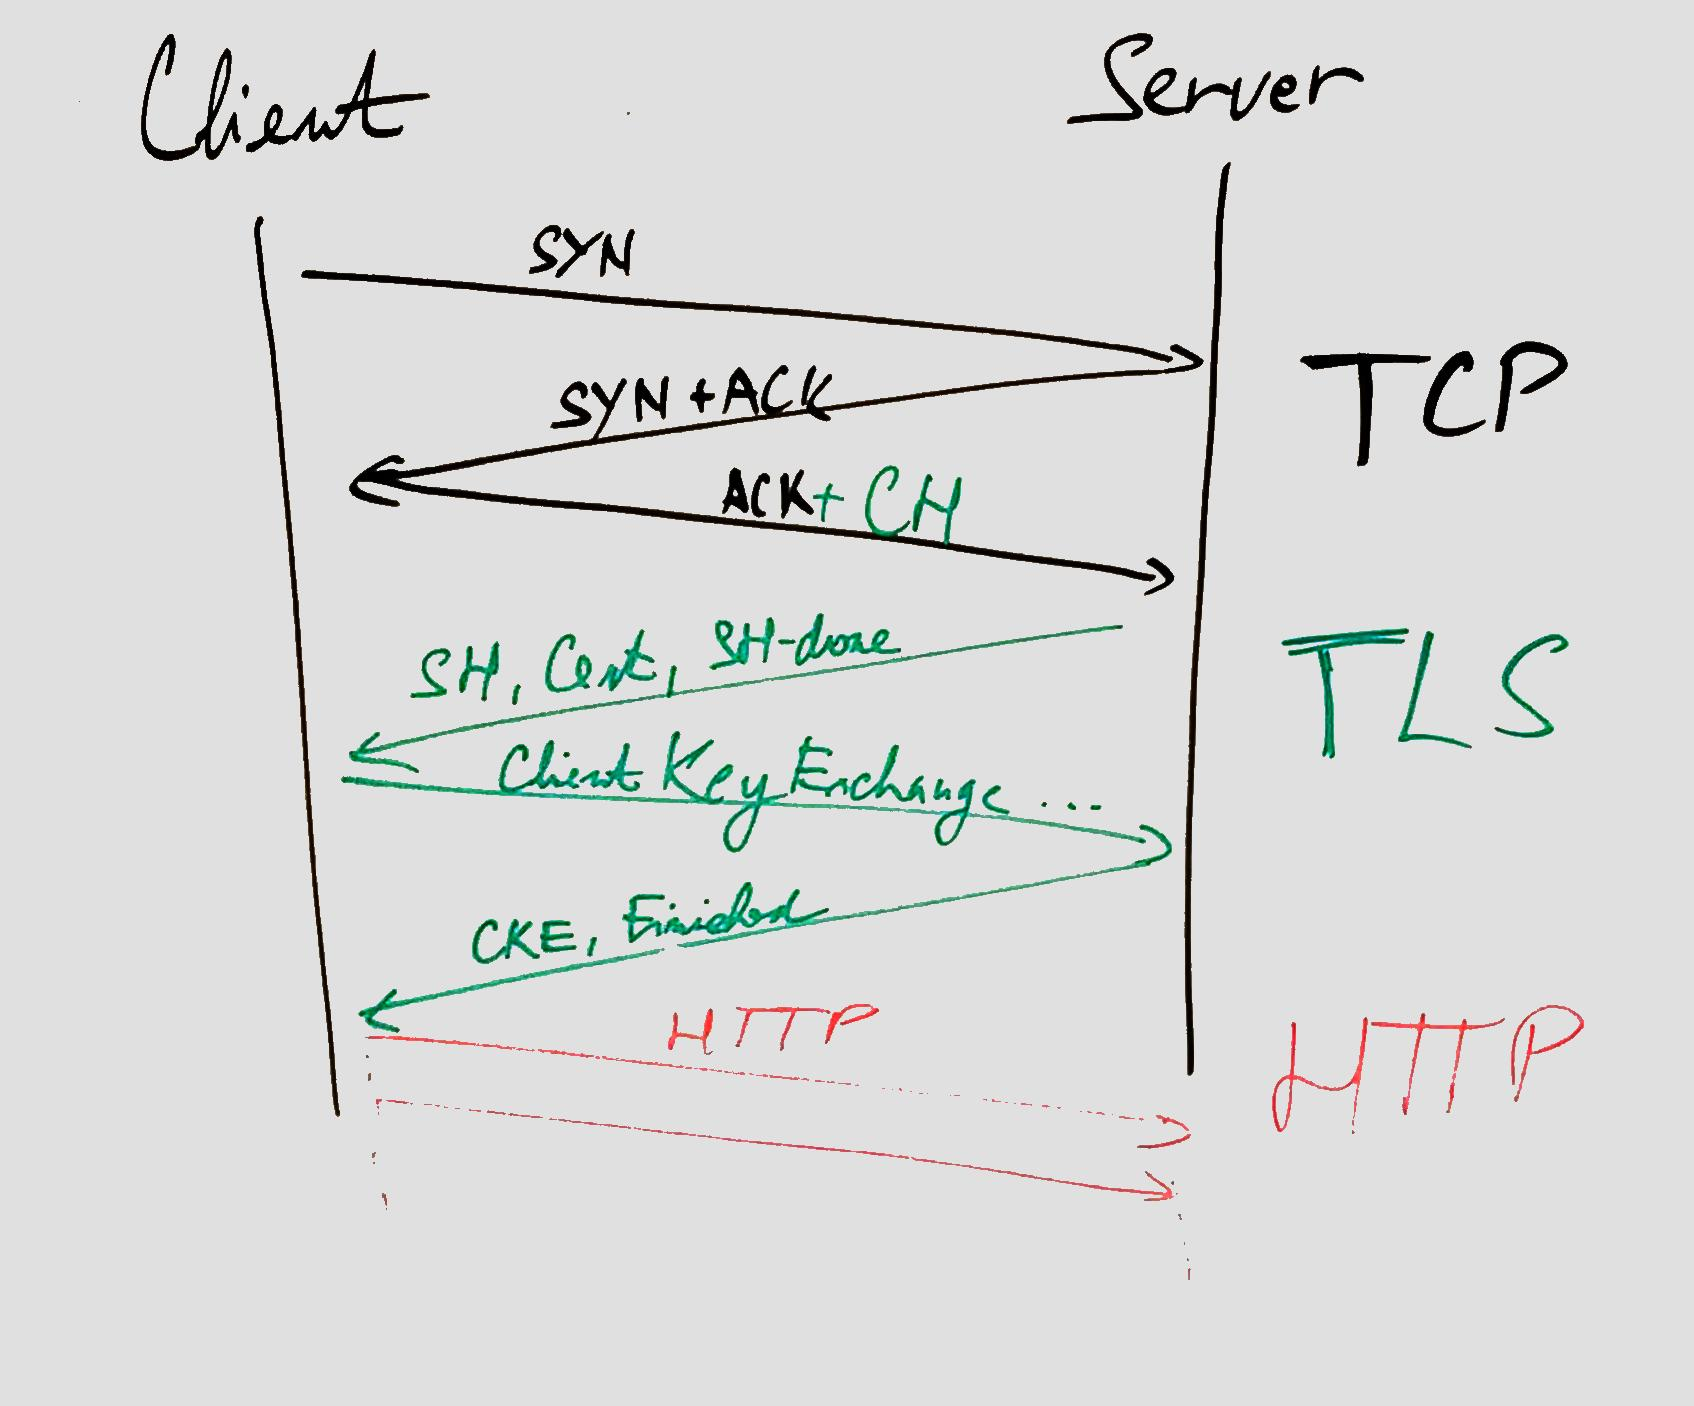
\includegraphics[width=0.6\textwidth]{img/01-https-connection-packets}
  \caption{Simplified view of the packets sent during HTTPS connection establishment}\label{fig:https-packets}
\end{figure}

More and more websites enforce the use of HTTPS to protect the privacy of their users. In August
2020, 96 out of top 100 viewed websites actively redirect to HTTPS, and more than 75\% of all
network traffic from Chrome web browser used HTTPS~\cite{googleTransparency}. With HTTPS becoming
the norm, almost all connections suffer from the increased latency incurred by the additional TLS
handshake.

\section{HTTP/3 and QUIC}

The next version of the HTTP protocol --- HTTP/3~\cite{draft-ietf-quic-http-29} --- addresses these
problems by replacing the TCP and TLS layer with brand new UDP-based protocol named
QUIC\footnote{Originally intended as the acronym for Quick UDP Internet Connection, but during
standartization QUIC has been changed to be the actual name of the protocol.}, and shifting
multiplexing capability from application to transport layer. The relationships between protocols on
HTTP/2 and HTTP/3 stacks are illustrated in figure~\ref{fig:http2-vs-http3-stack}.

\begin{figure}[h]
  \centering
  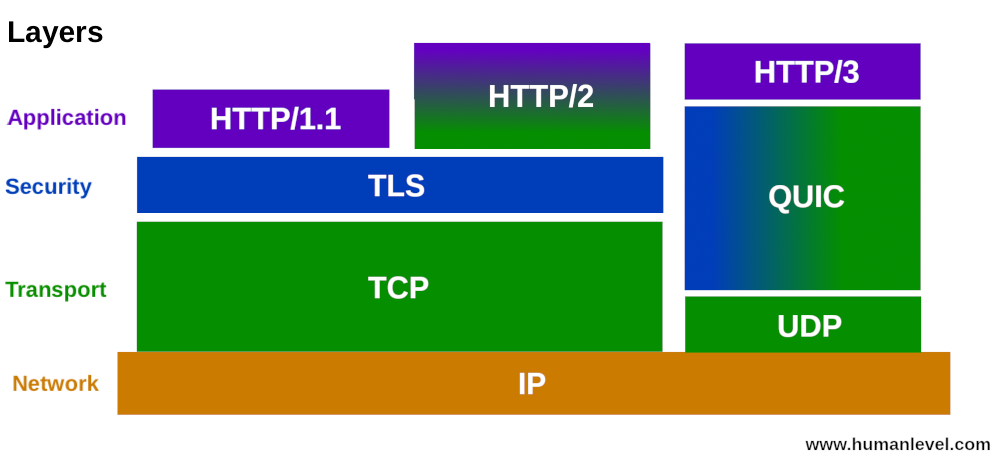
\includegraphics[width=\textwidth]{img/01-pile-http-protocol}
  \todo{Redraw this without HTTP/1.1 in inkscape, indicate which parts of the stack implement stream
    multiplexing, encryption, reliability etc.}
  \caption{Comparison between HTTP/2 and HTTP/3 protocol stacks}\label{fig:http2-vs-http3-stack}
\end{figure}

\todo{possibly more comments on the figure will go here}
Although QUIC development is tied with that of HTTP/3, it is designed as a general-purpose transport
layer protocol that can be used for other application level protocols as well. The main improvements
of QUIC over TCP+TLS can be summarized in following points:

\begin{itemize}
  \litem{Stream multiplexing}
    QUIC provides abstraction of multiple streams multiplexed on a single connection at the
    transport level. And because loss detection and retransmission is implemented also at the QUIC
    layer, rather than UDP, the protocol does not exhibit the \textit{head-of-line blocking}
    problem described above.

  \litem{Faster connection establishment} QUIC still performs TLS 1.3 handshake, but it does so in
    parallel with TCP-like three-way-handshake for the base protocol. This combined handshake
    requires fewer round-trips and therefore reduces latency. QUIC also supports TLS 1.3 Zero Round
    Trip Time Resumption (0-RTT for short). The 0-RTT mode of operation allows a client to cache
    some session information allowing it to send application data with the very first packet in
    future connection to the same server. This effectively reduces the latency by another round
    trip, but makes such requests vulnerable to repeat attacks. More detailed description of 0-RTT
    can be found online, e.g\@. on Cloudflare's blog~\cite{cloudflare-0rtt}.

  \litem{Always encrypted} TLS handshake is a mandatory part of connection establishment and
    therefore QUIC connections are always encrypted. This makes QUIC secure-by-default and no extra
    steps need to be taken by the application protocol to achieve security.

  \litem{Separating connection identity from peer's IP address} QUIC protocol does not use peers
    IP addresses to identify connections, but instead uses connection IDs which are 8 to 20 byte
    sequences negotiated during connection establishment. This makes QUIC very attractive for mobile
    devices, which can switch between multiple IP addresses. This happens e.g\@. when device
    switches from Wi-Fi to cellular data network. Ordinarily, the existing connection has to be
    terminated and new connection established from the new IP address. QUIC, on the other hand, can
    migrate the connections in a way that is transparent to the application layer.

    This feature also enables QUIC extensions like Multipath
    QUIC~\cite{draft-deconinck-quic-multipath-04}, which allows simulataneous use of multiple
    network interfaces for a single connection to achieve greater throughput.

\end{itemize}

As of August 2020, the specifications of HTTP/3 and QUIC are still at draft stage, but the
standartization process is believed to be very close to complete. There are already multiple
implementations of the draft versions of the standard and many of these implementations are backed
by big companies such as Google, Cloudflare, Facebook and Microsoft.

Experiments with these implementations allow early performance comparisons between HTTP/3 and
HTTP/2. In 2015 the experimental implementation by the Chromium team showed a 3\% improvement in
mean page load time and 30\% less rebuffer events when watching YouTube videos~\cite{Wilk2015}.
Cloudflare launched preliminary support for HTTP/3 in April 2020 and has measured 12.4\% decrease in
the \textit{time to first byte} metric~\cite{Tellakula2020}, which is consistent with the QUICs
promise of reduced latency. The QUIC protocol outperforms TCP especially in unstable networks such
as wireless mobile networks~\cite{Cook2017}.

\section{Support for QUIC in \dotnet{}}

Microsoft's \dotnet{} development team has long-term plans to provide full QUIC and HTTP/3 support
in \dotnet{}. In case of HTTP/3, the support should be completely transparent to users, because the
choice of protocol to be used is up to \texttt{HttpClient} class implementation.
Since QUIC can be used to build other protocols than HTTP/3, its implementation will be exposed via
public classes residing most likely inside the \texttt{System.Net.Quic} namespace.

The QUIC support has been originally intended for the \dotnet{} 5 release planned for November 2020.
However, it turned out that the standartization process wasn't going to be completed in time for
QUIC to be implemented for the release, so the work was interrupted and official HTTP/3 and QUIC
support was postponed for later releases.

\todo{probably remove the following subsection heading}

\subsection*{Existing QUIC Implementation in \dotnet{}}

The work-in-progress implementation of QUIC is still present in the master development branch of the
\dotnet{} runtime repository~\cite{dotnetGithub}, but has been made accessible only internally. This
implementation is a wrapper around the \libmsquic{} library~\cite{msquicGithub}, which is a C
implementation of QUIC developed by Microsoft. The \libmsquic{} library is designed for
high-performance scenarios and has been recently open-sourced.

Decision to use \libmsquic{} as the QUIC protocol implementation is not final. Using an existing
external implementation allows the development team to quickly evaluate the proposed QUIC API\@.
However, there are compelling arguments for implementing the QUIC protocol in managed \dotnet{} code
--- and more specifically, in \csharp{} --- for the production release.

% It is also cross-platform, with support for Windows and Linux operating systems.

\subsection*{Motivation for Implementing QUIC in Managed Code}

Code written in ahead-of-time compiled languages such as C or C++ (from now on reffered to as
\textit{native code}) is likely to be faster than code written in \dotnet{} languages (from now on
referred to as \textit{managed code}), which rely on just-in-time compilation. However, there are
other aspects than raw performance to be considered when deciding to use native libraries such as
\libmsquic{}:

\begin{itemize}

  \litem{Cross-platform compatibility/availability} The \dotnet{} platform officially supports
    multiple versions of Windows, macOS and several Linux distributions. If the native library does
    not support all these platforms, then an alternative library has to be used on other platforms,
    introducing more complexity into the codebase.

  \litem{Support for different library versions} Currently, no native libraries that managed
    \dotnet{} libraries depend on are part of \dotnet{} distribution. Instead, it is expected that
    the library is already installed on the target machine and can be dynamically loaded. This means
    that the \dotnet{} code must work correctly with multiple different versions of the native
    library.

  \litem{Maintainability} Maintenance of the interop code requires the developer to be able to
    read and understand the language in which the native library is written. Debugging the code
    around the language boundaries may be difficult in case the necessary tooling for mixed-language
    debugging is not available.

  \litem{Library's API} One of the aspect greatly influencing the resulting performance is
    similarity between the public API of the \dotnet{} library and the API of the native library in
    question. The relevant aspects are whether the API are following:

    \begin{itemize}
      \item Event-based (i.e\@. using callbacks) vs\@. method based
      \item Blocking vs\@. non-blocking
      \item Synchronous vs\@. asynchronous
      \item Which side allocates memory buffers
    \end{itemize}

    The interop layer of the code needs to translate the necessary differences, which may incur
    noticeable performance overhead and even negate the performance gained from the use of native
    library.

  \litem{Future development} Implementing new features requires prior support in the native
    library, and becuase the use of newer library versions cannot be enforced, the features must be
    designed as optional in \dotnet{}.

\end{itemize}

In the past, the \dotnet{} team has encountered multiple problems with the
\libcurl~\cite{curlGithub} library, which was used to implement HTTP request handling. Different
Linux distributions contain different versions of the \libcurl{} library, with different features as
well as different bugs. The dotnet{} development team had to expend a lot of resources to make sure
the managed code written by \dotnet{} developers behaved consistently on all platforms.

Starting with \dotnet{} Core 2.1, the default implementation of HTTP request handling does not rely on
native libraries like \libcurl{}. Instead, the functionality has been rewritten in pure managed
code, which offered better performance and consistent behavior across all \dotnet{}
platforms~\cite{SocketsHttpHandlerDocs}.

The reasons above motivated Microsoft developers to decide that it would be better to have managed
implementation of the QUIC protocol and avoid adding native dependencies.

\section{Goals of this Thesis}

This thesis seeks to create a partial implementation of QUIC, which could be used as the basis of
the future official \dotnet{} implementation. The result of this thesis should be compilable branch
of the \dotnet{} runtime, which exposes the QUIC API for other \dotnet{} developers to use.

Although managed code should be portable, the API for working with TLS 1.3 that is necessary for
implementing QUIC is currently unavailable in \dotnet{}. In order to avoid implementing TLS 1.3
ourselves, the managed QUIC implementation will still require a native TLS 1.3 library. The
future managed implementation would use different library to implement TLS 1.3 on different
operating systems, but for the purposes of this thesis it will be sufficient to use the same library
on all platforms.

The existing QUIC implementation in \dotnet{} uses a layer of indirection, allowing multiple
implementations exist side by side, and possibly switching betwen them at program runtime. This
thesis will add the managed QUIC implementation alongside the \libmsquic{}-based one, and allow for
comparison between them.

We have mentioned that the design of the QUIC API was interrupted early. The current version does
not expose all features of the QUIC protocol. However, the current API should be sufficient for
implementing simple application protocols on top of QUIC\@. This thesis will therefore avoid making
any modifications to the API\@.

Implementing the full QUIC specification is outside the scope of a master thesis. Fortunately, some
parts of the specification are concerned with aspects that need not come into effect for many
connections, and can be therefore omitted from our prototype implementation. For example, most QUIC
connections are not likely to use the connection migration feature. Because we do not expect readers
to be fully familiar with the QUIC protocol specification and all its features, we will present an
overview of the protocol in Chapter~\ref{chap:02-quic} and defer selection of the protocol features
to be acutally implemented as part of this thesis to the beginning of the analysis in
Chapter~\ref{chap:03-analysis}. The design of the implementation, however, should be such that the
rest of the specification can be implemented in the future.

It would make sense to evaluate functionality of our QUIC implementation by providing also partial
implementation of HTTP/3. However, even supporting the simplest GET requests would be too
complex. Instead, we will implement a primitive client-server console application. The client part
of the application will send all files in a given directory to the server, which will store them.
The files will be sent in parallel, utilizing the stream multiplexing feature of QUIC\@.

Because the motivation behind QUIC is to improve performance over using the combination of TCP+TLS,
this thesis should also try to compare the performance of these protocols when used from \dotnet{}
via a set of benchmarks.

\subsection*{Summary of the Goals}

The following list summarizes the goals of this thesis presented in previous subsection.

\begin{enumerate}
  \item Select sufficient subset of QUIC specification needed support basic data transfer and
    implement it.

  \item Make the existing QUIC API publicly accessible, and allow switching between the new managed
    implementation and the existing \libmsquic{} based one.

  \item Evaluate the QUIC implementation by implementing a simple client-server console application
    for sending files.

  \item Try to compare the performance of the new implementation with the previous msquic-based one.

\end{enumerate}
